% !TeX encoding = UTF-8
% !TeX spellcheck = fr-classique
%% NOTES :
% Pour reindenter le fichier :
% latexindent rapport_TER.tex -o rapport_TER.tex


\documentclass{report}
\usepackage{fontspec}
\usepackage{microtype}
\usepackage{lmodern}
\usepackage{tabu}

\usepackage{polyglossia}
\setmainlanguage{french}


\usepackage{float}

%\usepackage{breqn}
\usepackage{amsmath}

\usepackage[hidelinks]{hyperref}

\usepackage{minted}
\usepackage{tikz}
\usetikzlibrary{positioning}

\title{Rapport UE Apprentissage statistique : Réconnaissance d'images}
\author{Nicolas \textsc{Leclerc} \and Damien \textsc{Gabriel} \and Mohammed \textsc{Boutahar}}
\date{M1 Informatique 2015-2016}

\begin{document}

{\let\newpage\relax\maketitle}

\begin{tikzpicture}[remember picture, overlay]
%\node[anchor=north east, inner sep=20pt] at (current page.north east) {
\includegraphics[width=2cm]{images/logo_saclay.png}};

\node[anchor=north west, inner sep=20pt](upsud) at (current page.north west) {
\includegraphics[width=2cm]{images/logo_upsud.png}};
%\node[below = -1cm of upsud] {\includegraphics[width=2cm]{images/logo_LIMSI.png}};

%\node[anchor=north east, inner sep=20pt] at (current page.north east) {\includegraphics[width=2cm]{images/logo_LIMSI.png}};
\end{tikzpicture}

\tableofcontents

%% Introduction
\chapter{Introduction}

Pour un humain, la classification des images est assez facile sur des images bien définies, ce qui est le cas du CIFAR-10.

Il est intéressant de pouvoir classifier automatiquement des images, ou de  façon plus générale, de pouvoir extraire des informations automatiquement d'un ensemble de données. On peut imaginer de nombreuses applications comme par exemple la création automatique de légende pour des images ou encore l'identification de personnes.

%% CIFAR
\chapter{CIFAR-10}


La base CIFAR-10 est une base d'images de petites taille contenant 60000 images de 32 * 32 pixels. Ces images sont réparties dans 10 classes (avions, voiture, oiseau, chat, biche, chien, grenouille, cheval, bateau et camion), chacune contenant 6000 images.

Il y a 6 lots de données répartis en 5 d'apprentissage et 1 de test.

Le lot de test contient 10000 images avec 1000 images sélectionnées dans chaque classe. Les lots d'entrainement contiennent le reste.

Il n'existe pas de recouvrement entre les classes, elles sont mutuellement exclusives.


Les données peuvent être récupérées sous différents format. Dans le cadre d'une utilisation avec \texttt{python}, on utilisera des fichiers produits par cPikle, qui permettent d'obtenir un dictionnaire de la forme :

\begin{itemize}
\item[clé : data] 10000x3072 d'entier non signés 8 bit (0-255). Chaque ligne contient une image 32 * 32 pixels. Les canaux sont ensuite dans l'ordre R (rouge), G (vert), B (bleu), chaque canal a 1024 (32 * 32) éléments. Les images sont stockées par lignes.

\item[clé : label] 10000 contient un nombre de 0 à 9 permettant de connaitre la classe des 10000 images.
\end{itemize}

La page \url{http://rodrigob.github.io/are_we_there_yet/build/classification_datasets_results.html} contient les meilleurs résultats obtenu sur la base CIFAR-10. 

Actuellement le taux de reconnaissance atteint 96.53~\% \cite{DBLP:journals/corr/Graham14a}.

Il est très peu probable que nous atteignons un tel taux de reconnaissance. En effet, ceux-ci suppose des algorithmes complexes avec des réseaux de neurones  comme dans \cite{DBLP:journals/corr/Graham14a}. Le temps limité ne nous permettra pas d'implémenter et de trouver les meilleurs paramètres pour obtenir les meilleurs résultats.

Un autre problème sera la puissance de calcul disponible qui ne permettront pas de traiter un très grand nombre d'images d'apprentissage.




\chapter{Méthode naïve}

Dans un premier temps, on utilisera comme caractéristique les valeurs de chaque pixel.

On peut utiliser comme valeur des pixels la «norme» des composantes R, G, B
avec~:

\begin{itemize}
\item R : la composante rouge de l'image
\item G : la composante verte
\item B : la composante bleu
\end{itemize}

Avec cette définition de la valeur, $val$ des pixels, celle-ci peut s'écrire :

\begin{equation}
val = \sqrt{R^{2} + G^{2} + B^{2}}
\end{equation}

Ci-dessous on présente les résultats obtenus en utilisant la totalité du \verb|data_batch1| et du \verb|test_batch|.

Plusieurs cas on été réalisés :
\begin{itemize}
\item Le perceptron non moyenné et sans shuffle sur 100 périodes
\item Le perceptron non moyenné avec shuffle sur 100 périodes
\item Le perceptron moyenné avec shuffle sur 100 périodes
\item La k-moyenne sur 30 périodes
\end{itemize}

\section{Perceptron}

Le perceptron est un séparateur linéaire permettant de classifier avec supervision de manière binaires des images.

Pour une entrée $x$ on renvoit soit 0 ou 1 (ou -1 et 1) selon la valeur du produit scalaire entre les poids $w$ et le vecteur d'entrée  est supérieur à un seuil $b$.

\begin{itemize}
\item si $w.x + b > 0$ : $f(x) = 1$ 

\item sinon    $f(x) = 0$ 

\end{itemize}

Si la valeur retournée est positive alors on considère que x appartient a cette classe.

Si la valeur retournée est nulle alors x n'appartient pas à la classe considéré.

Dans le cas d'un perceptron multiclasse, on utilise un perceptron pour chaque classe.

Dans un premier temps on fait «apprendre» à l'algorithme à reconnaitre les images dont on connait déjà la classe. On procède de manière itérative en déterminant les poids associé à un vecteur de caractéristique afin de minimiser les erreurs de prédiction. Les vecteurs de caractéristiques sont créés de façon à représenter les objets de l'on manipule. Par exemple, dans le cas d'image, on peut utiliser des valeurs associée aux pixels telle que la norme avec différents regroupements.


\subsection{Non moyenné et sans shuffle}

La figure ci-dessous représente, pour chaque classe, le nombre d'image mal reconnues en fonction de la période.

Chaque classe contient 1000 images, ce qui nous permet de comparer directement le taux de reconnaissance de chaque classe.

Globalement, le nombre d'erreur est important et même dans le cas des images représentant des avions et des bateaux, qui sont les classes les mieux reconnues, on n'a qu'environ 300 images reconnues correctement. Soit un taux de reconnaissance d'environ 30 \%.

On peut penser que la faible variabilité de la couleur du ciel et de la mer, dans le cas des images d'avions et de bateau, permet de les identifier facilement, une fois qu'un l'on connait la couleur de base. Ainsi un processus basé sur l'utilisation de couleur (par opposition à une détection de contour) est elle suffisante. Au contraire, on peut penser, pour les classes mal reconnues, que la variabilité des couleurs est trop forte pour pouvoir identifier correctement une image uniquement à l'aide de la norme euclidienne des composantes R,G,B des pixels.

De même la composition des images ne sera pas identique. Autant un avion ou un bateau sera très souvent sur un fond relativement uni, autant une photo de la classe cerf aura pour fond une forêt avec de fortes variations de couleur autour du cerf. 

% TODO insérer image

On observe une convergence de chaque classe bien que pour certaines le taux de d'images mal reconnues soit croissant. En effet il se peut que l'algorithme prédisait trop souvent ce type d'image ce qui implique qu'il se trompait souvent sur les autres classes et non sur la classe prédite.

\begin{figure}[H]
\begin{center}
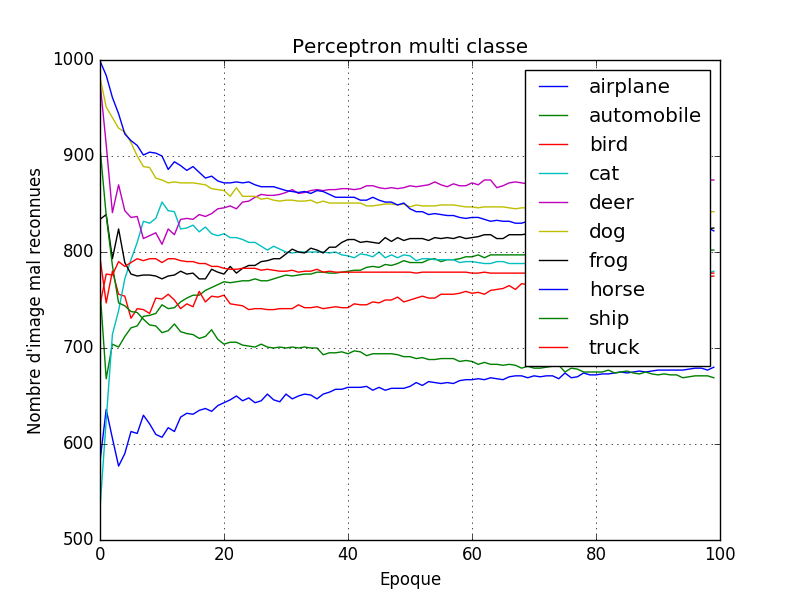
\includegraphics[width=\textwidth]{images/Perceptron_multiclasse_non_moyenne.png}
\caption{Nombre d'images mal reconnues pour chaque période et pour chaque classe pour le perceptron non moyenné et sans shuffle}
\end{center}
\end{figure}

La figure suivante représente le taux d'erreur global pour les différentes périodes.
Au cours des période le taux d'erreur global diminue et tend à se stabiliser bien que lentement. Il reste en dessus du taux sur l'apprentissage puisque les jeux de données sont distincts.

\begin{figure}[H]
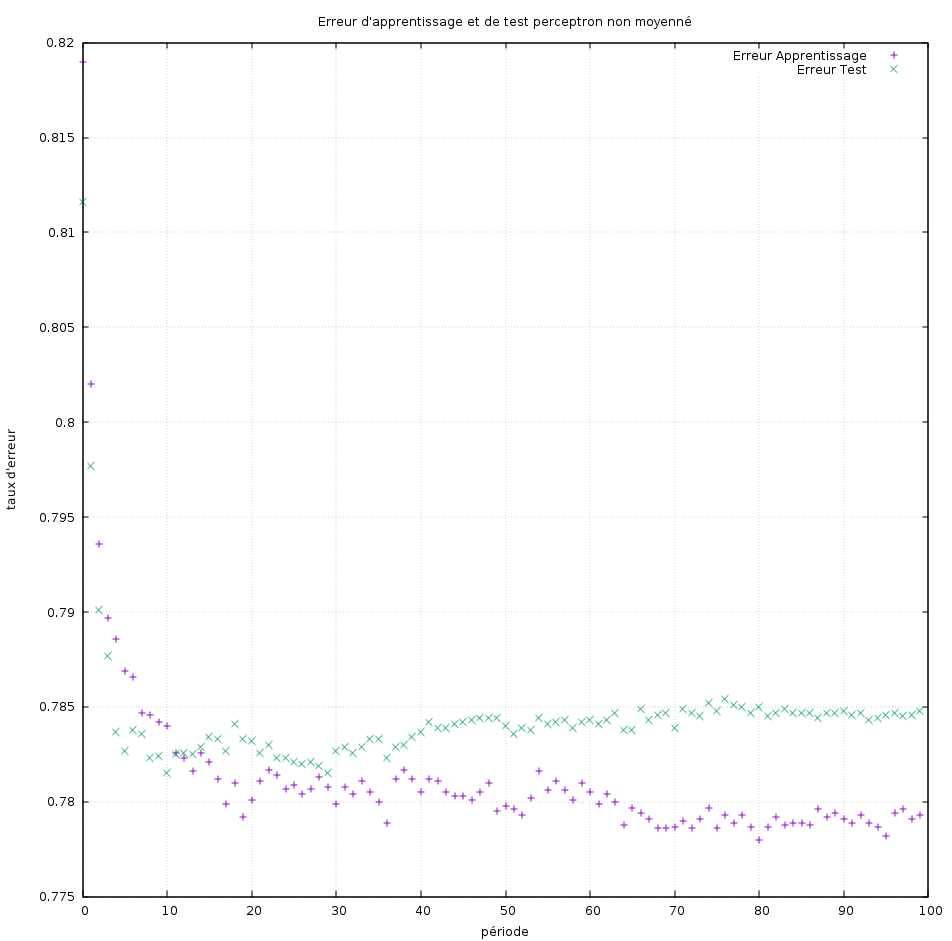
\includegraphics[width=\textwidth]{images/erreur_Perceptron_multiclasse_non_moyenne.png}
\caption{Taux d'erreur global, perceptron non moyenné sans shuffle}
\end{figure}


\subsection{Non moyenné avec shuffle}

La figure \ref{fig:perceptron-non-moyenne-shuffle} représente le nombre d'images mal reconnues, pour chaque classe au cours des différentes périodes.
L'atout du shuffle est de minimiser le poids du ou des dernières itérations de l'apprentissage par une(des) image(s) trop singulières. Les résultats sont sensiblement meilleur bien que très variables car les images de fin d'apprentissage varient elles aussi.

\begin{figure}[H]
\begin{center}
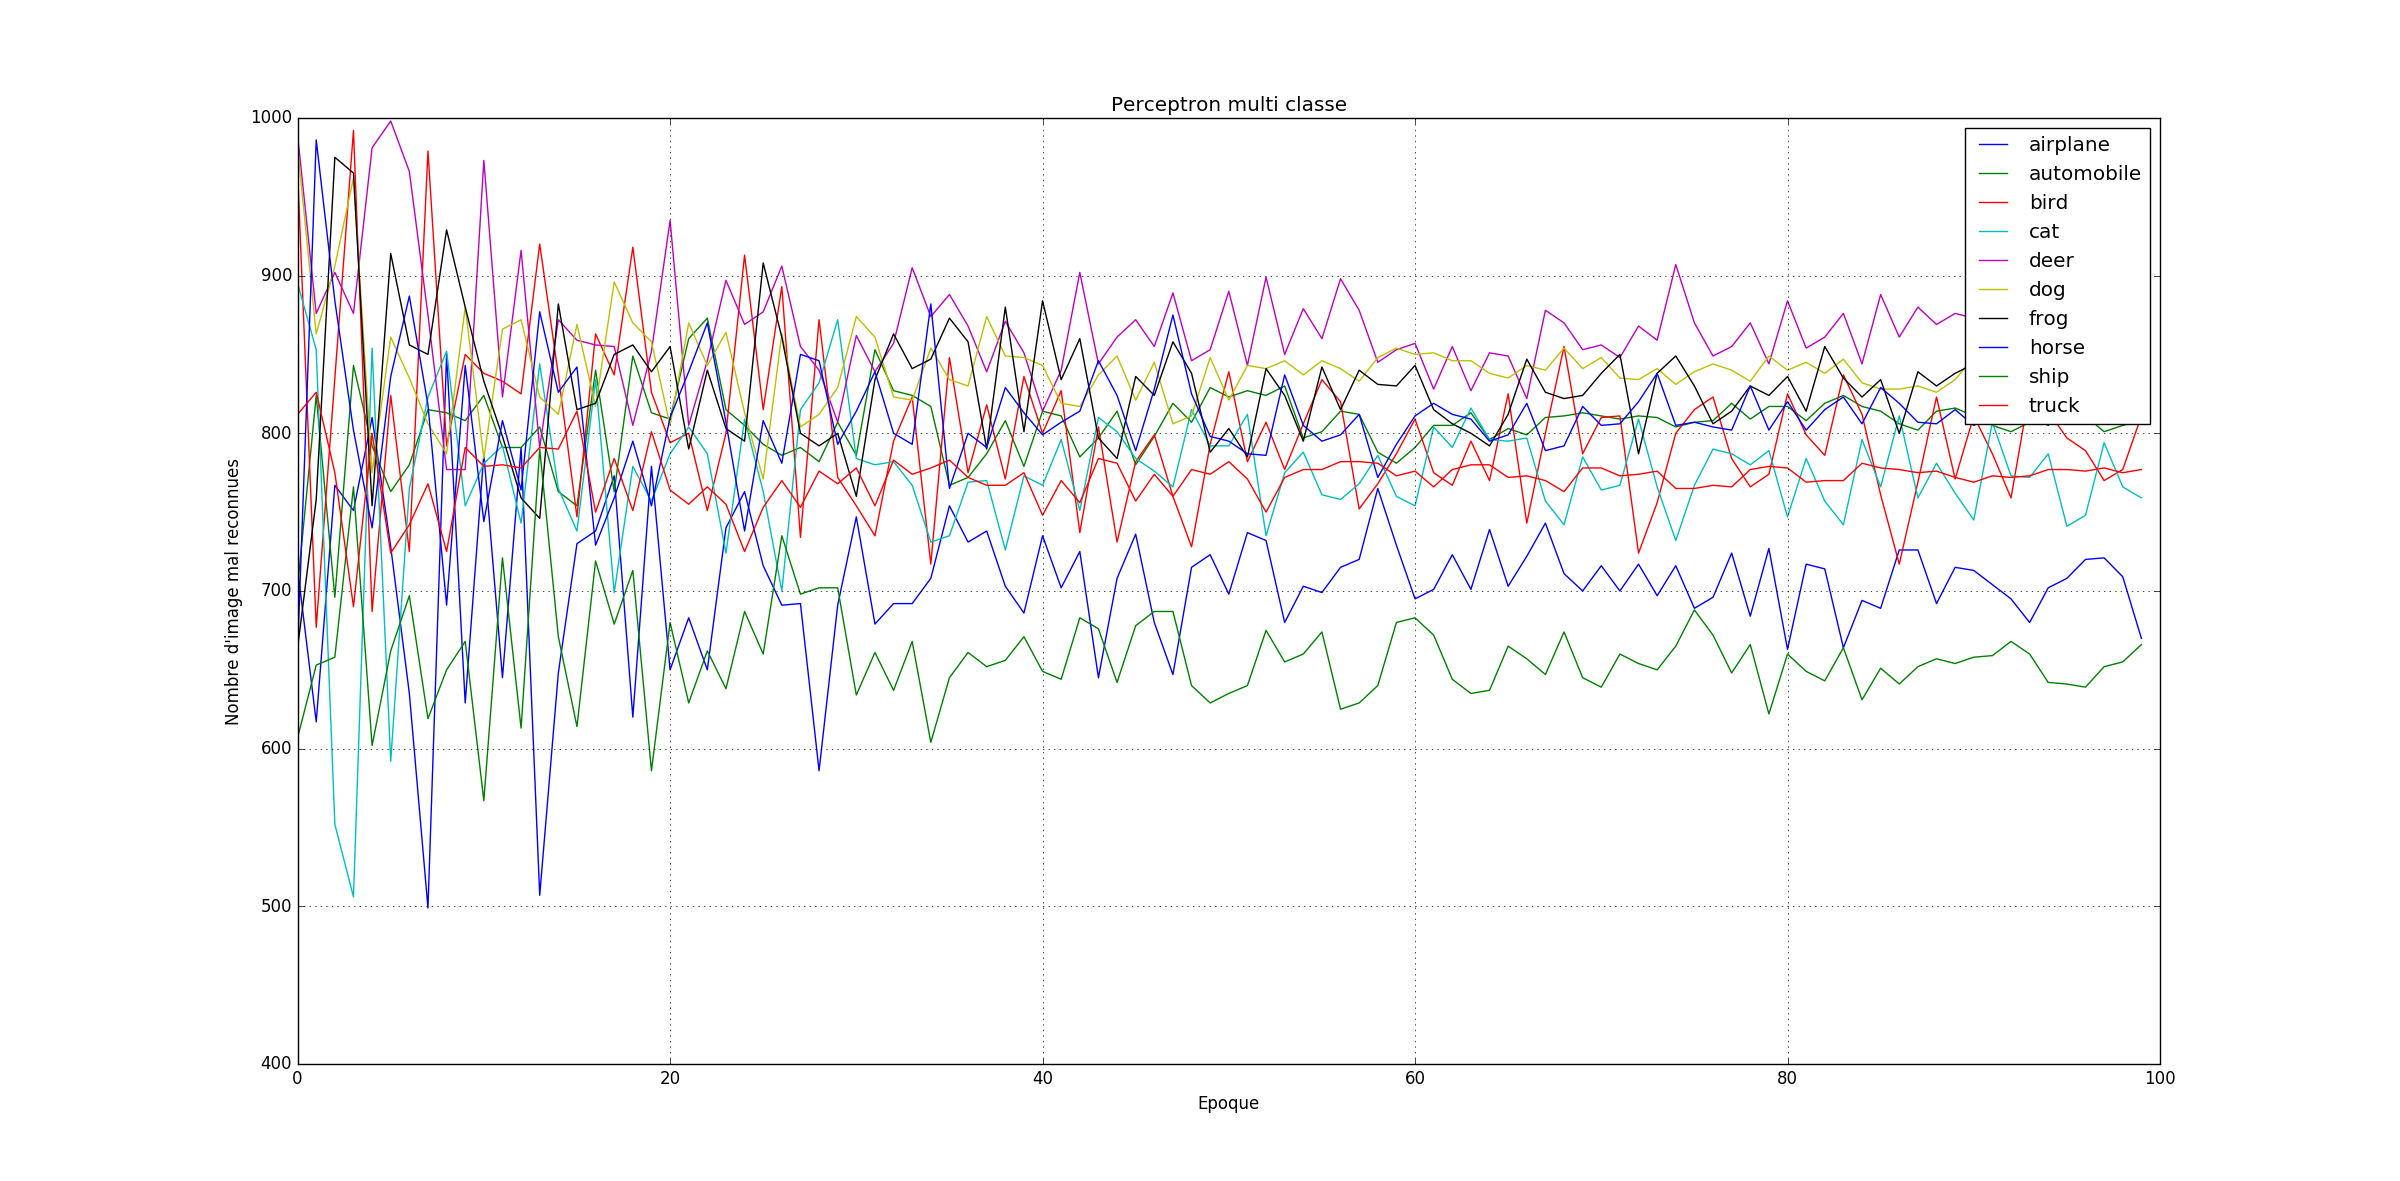
\includegraphics[width=\textwidth]{images/Perceptron_multiclasse_non_moyenne_shuffle.png}
\caption{Nombre d'images mal reconnues pour chaque période et pour chaque classe pour le perceptron non moyenné avec shuffle}
\label{fig:perceptron-non-moyenne-shuffle}
\end{center}
\end{figure}

La figure \ref{fig:erreur-perceptron-non-moyenne-shuffle} représente le taux d'erreur global pour les différentes périodes.

\begin{figure}[H]
\begin{center}

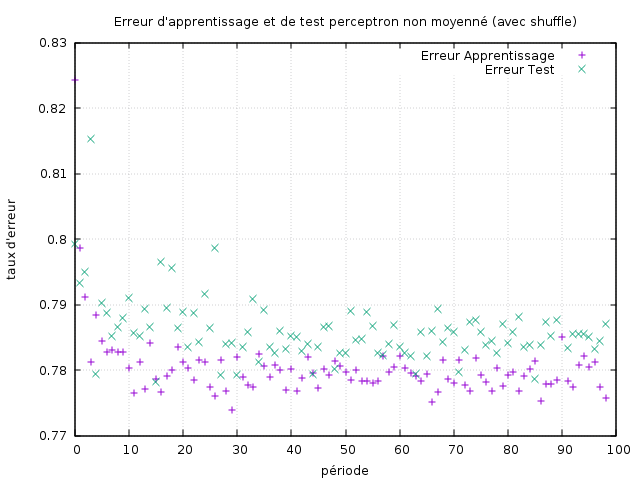
\includegraphics[width=\textwidth]{images/erreur_Perceptron_multiclasse_non_moyenne_shuffle.png}
\caption{Taux d'erreur global, perceptron non moyenné avec shuffle}
\label{fig:erreur-perceptron-non-moyenne-shuffle}
\end{center}
\end{figure}

\subsection{Moyenné avec shuffle}

La figure \ref{fig:perceptron-moyenne-shuffle} représente le nombre d'images mal reconnues, pour chaque classe au cours des différentes périodes.
Afin de supprimer la variantion trop important apporté par le suffle, nous utilisons un perceptron moyenné. Cela permet d'ammortir les changements de modèles du perceptron lors d'images trop singulières.

\begin{figure}[H]
\begin{center}


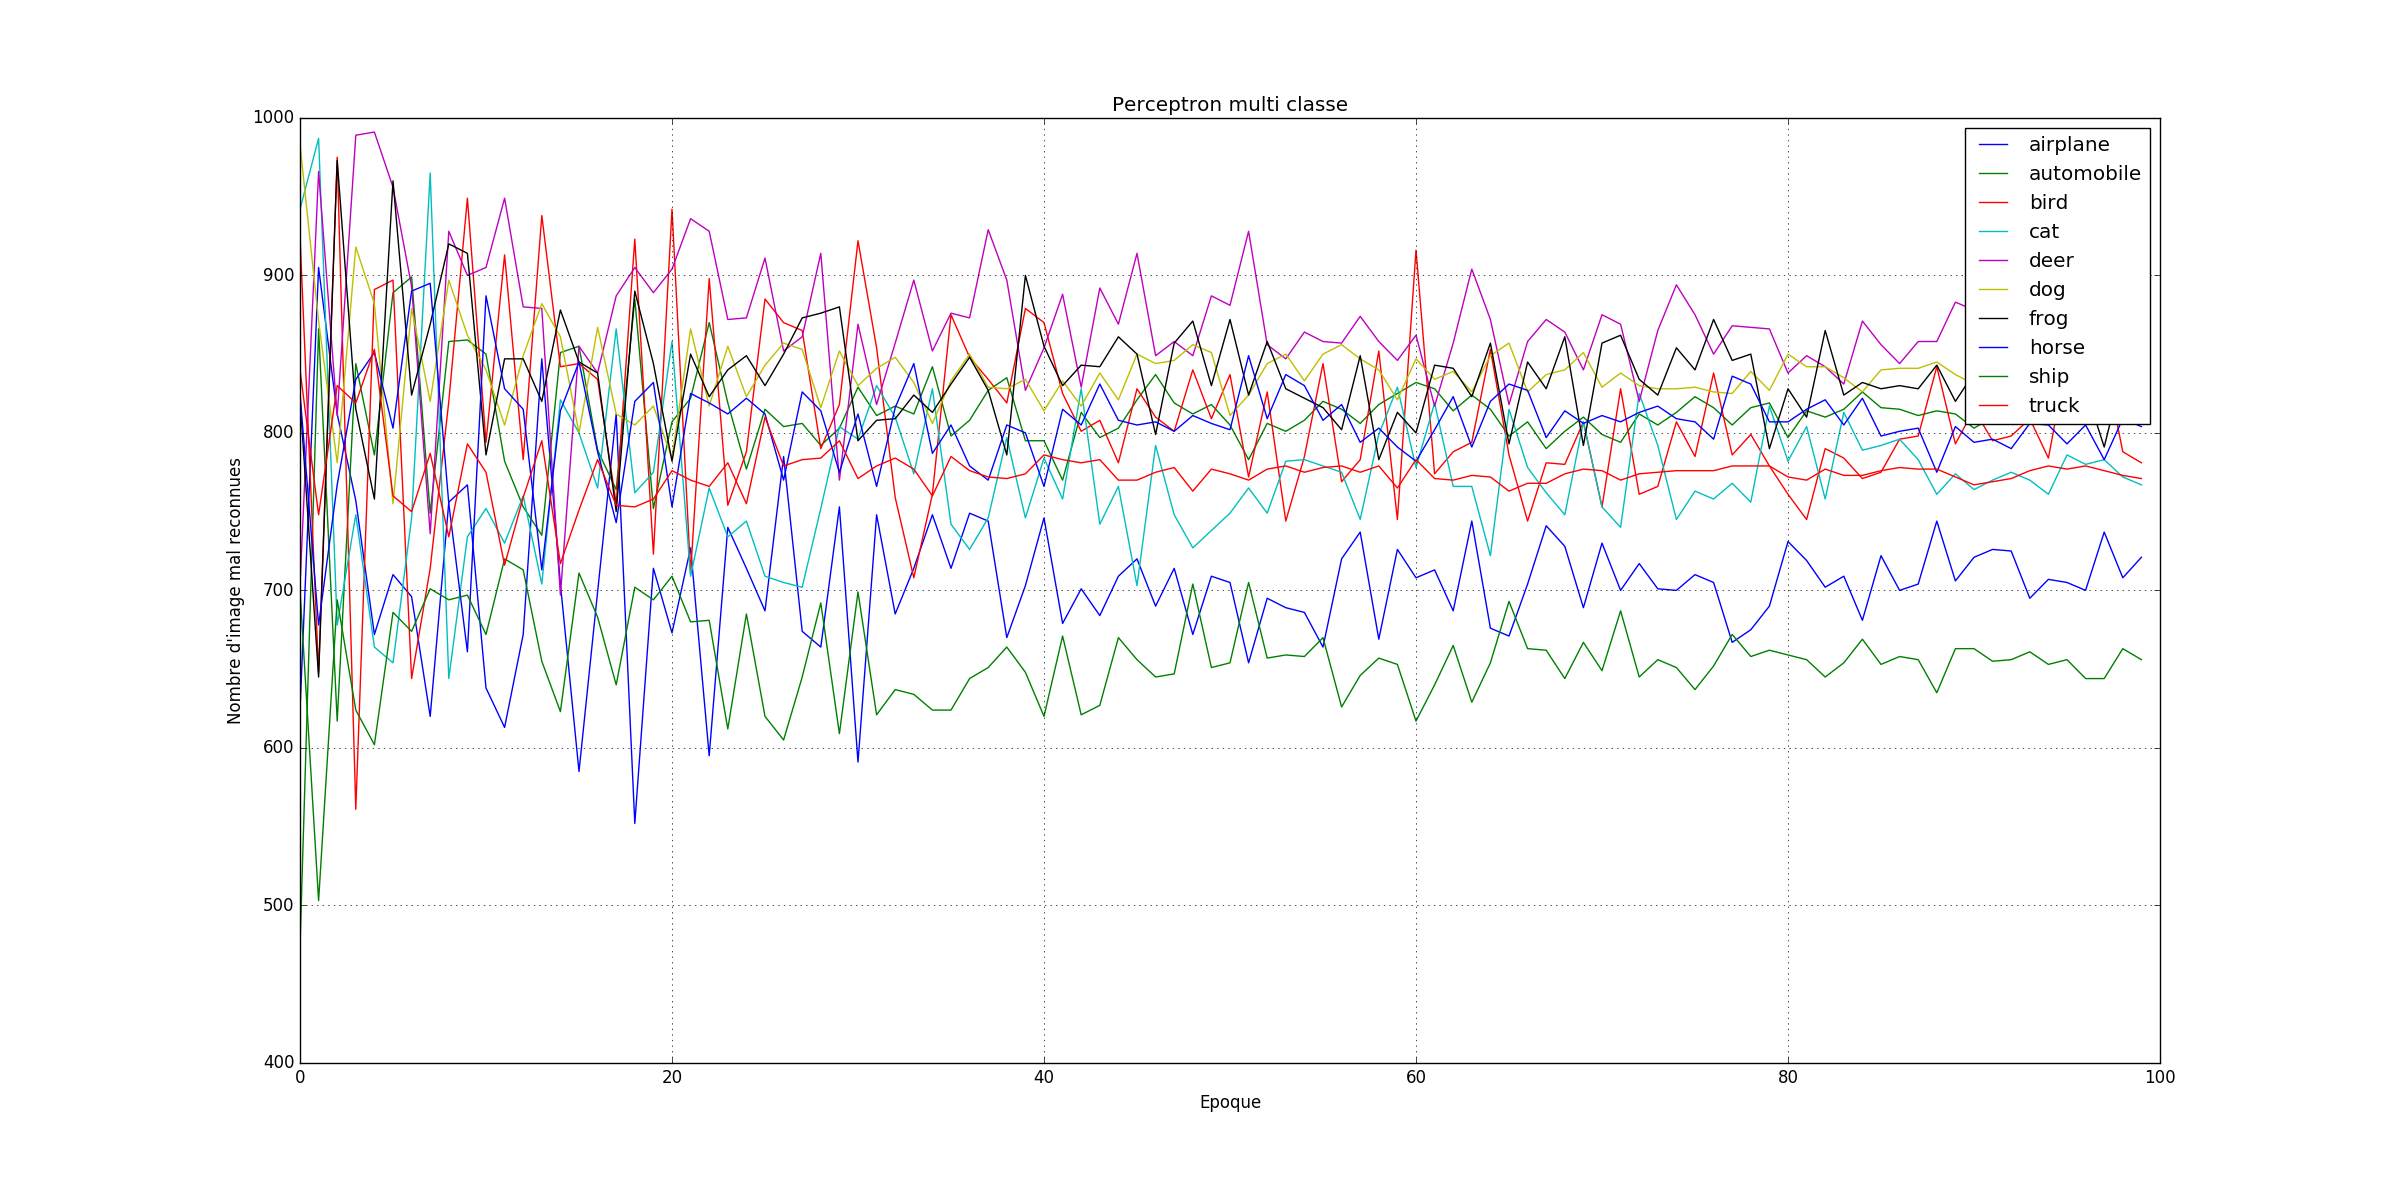
\includegraphics[width=\textwidth]{images/Perceptron_multiclasse__moyenne_shuffle.png}
\caption{Nombre d'images mal reconnues pour chaque période et pour chaque classe pour le perceptron moyenné avec shuffle}
\label{fig:perceptron-moyenne-shuffle}
\end{center}
\end{figure}

La figure \ref{fig:erreur-perceptron-moyenne-shuffle} représente le taux d'erreur global pour les différentes périodes.

\begin{figure}[H]
\begin{center}

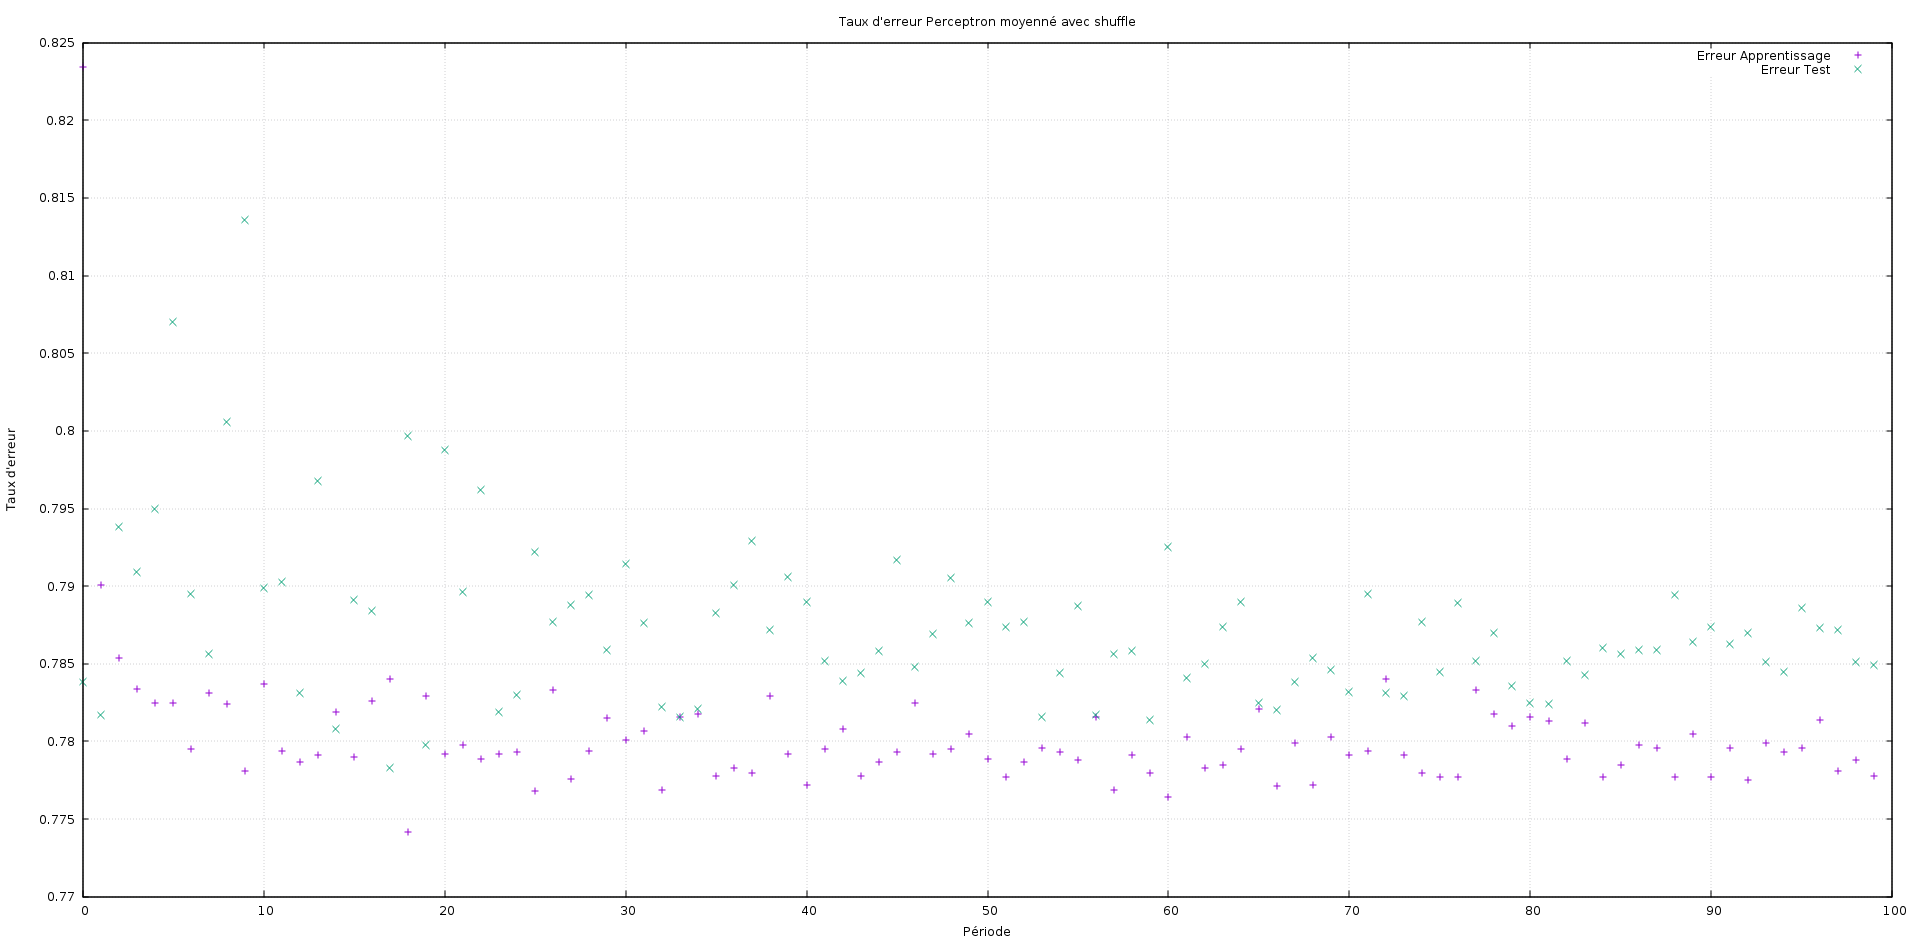
\includegraphics[width=\textwidth]{images/erreur_Perceptron_multiclasse_moyenne_shuffle.png}
\caption{Taux d'erreur globale, perceptron moyenné avec shuffle}
\label{fig:erreur-perceptron-moyenne-shuffle}
\end{center}
\end{figure}


\begin{figure}[H]
\begin{center}
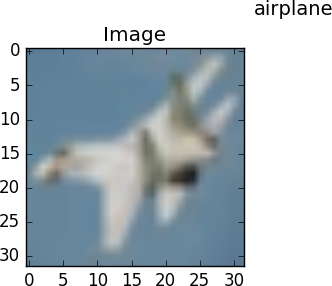
\includegraphics[width=0.4\textwidth]{images/avion_1.png}
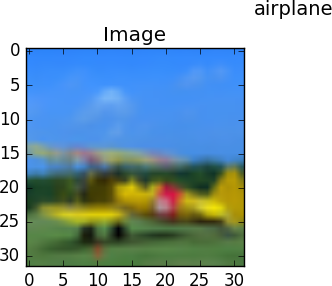
\includegraphics[width=0.4\textwidth]{images/avion_2.png}
\caption{Deux images de la classe «airplane» : noter la composition homogène de la partie supérieure de l'image. De même le ciel ne présente pas une grande différence de teinte}
\end{center}
\end{figure}


\begin{figure}[H]
\begin{center}
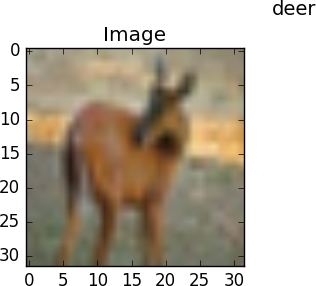
\includegraphics[width=0.4\textwidth]{images/deer_1.png}
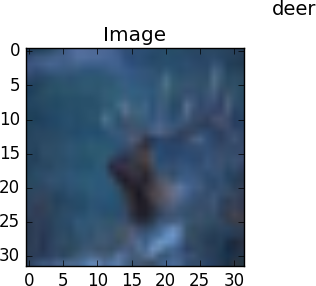
\includegraphics[width=0.4\textwidth]{images/deer_2.png}
\caption{Deux images de la classe «deer» : noter la grande différence de couleur de fond entre les deux images}
\end{center}
\end{figure}

\subsection{K-moyennes}
L'algorithme des k-moyennes n'étant pas supervisé les résultats obtenus ne permettent pas de classer les images. La prédiction est loin d'être satisfaisante (près de 90 \% de taux d'erreur).
On peut cependant améliorer ses performances avec des centroïdes initiaux bien choisis. Malheureusement, avec notre choix de distance basée sur les valeurs de pixel, ainsi que les données des images non traitées, il n'est pas possible de créer des centroïdes représentatifs d'une classe.

\begin{figure}[H]
\begin{center}
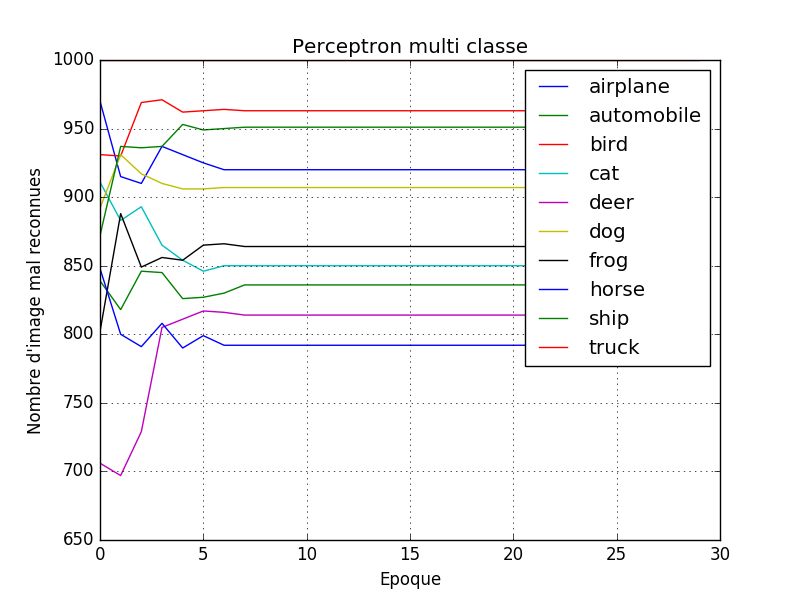
\includegraphics[width=\textwidth]{images/k-moyennes.png}
\caption{Nombre d'images mal reconnues pour chaque période et pour chaque classe pour la k-moyenne}
\label{fig:k_moyenne}
\end{center}
\end{figure}

\begin{figure}[H]
\begin{center}
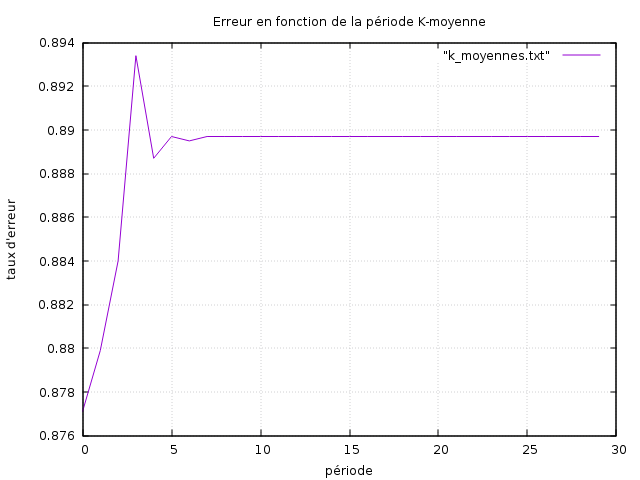
\includegraphics[width=\textwidth]{images/erreur_k_moyenne.png}
\caption{Taux d'erreur globale pour la k-moyenne en fonction de la période}
\label{fig:erreur-k-moyenne}
\end{center}
\end{figure}


\chapter{Apprentissage de caractéritiques}

L'apprentissage de l'approche naïve (valeur de pixels) ne permet pas d'extraire les caractéristiques d'une image. L'extraction de caractéristique est un important pas dans l'apprentissage afin de mieux classifier les images par la suite.

Adam Coates, Honglak Lee et Andrew Y. Ng font part de leur méthode d'extraction de caractéristiques dans leur arcticle « An Analysis of Single-Layer Networks in Unsupervised Feature Learning » \cite{coates2011analysis}. La méthode repose sur les étapes suivantes :

\begin{itemize}

\item Extraire des patchs de chaque image du corpus d'apprentissage.
	\item Collecter l'ensemble des patchs.
\item Appliquer une étape de prétraitement sur les patchs (normaliser et réorganiser les données)
	\item Appliquer un algorithme non supervisé tel que le k-moyenne sur les patchs afin d'en extraire des caractéristiques.
	\item Organiser les patchs selon un vecteur de caractéristiques.
	\item Appliquer un algorithme d'apprentissage.
	\item Extraire de même des patchs, les collecter, les pré-traiter, et les organiser selon un vecteur de caractéristiques pour les images du corpus de test.
	\item Appliquer un algorithme de classification.

	\end{itemize}

	Nous avons donc procédé tel quel avec un nombre de patchs égal à quatre. Afin d'extraire des caractéristiques nous utilisons un algorithme de k-moyenne. Ensuite pour la phase d'apprentissage et de classification nous utilisons SVC (Support Vector Classification) , un algorithme supervisé.

	Il faut noter que les problèmes de performances qu’entraîne le pré traitement est notable mais est aussi une étape fondamentale dans la méthode.

	Comme dit dans le k-moyenne, l'algorithme est très sensible à l'image référence de départ pour chaque classe. Cela donne des résultats très aléatoires. On a donc utilisé un shuffle afin d'observer les différents résultats pouvant être obtenus.
	Cette approche est cependant assez satisfaisante bien que les performances ne dépassent pas 70 \% de reconnaissance. En effet le faible nombre de patchs utilisés ne permet pas de capturer assez de caractéristiques.


%% Bibliographie

% TODO : ajouter les références des articles sur les formulations

\bibliographystyle{plain}
\bibliography{biblio/biblio_IA-APP}

\chapter*{Annexes : codes utilisées}

Voir les pièces-jointes

% Code utilisé pour le perceptron
%\inputminted{python}{codes/k-moyennes.py}

% Code utilisé pour la k-moyenne
%\inputminted{python}{codes/perceptron_multi_classe_moyennes.py}



\end{document}

